\documentclass[conference]{IEEEtran}
\usepackage{cite}
\usepackage{amsmath,amssymb,amsfonts}
\usepackage{algorithmic}
\usepackage{graphicx}
\usepackage{textcomp}
\usepackage{xcolor}
\def\BibTeX{{\rm B\kern-.05em{\sc i\kern-.025em b}\kern-.08em
    T\kern-.1667em\lower.7ex\hbox{E}\kern-.125emX}}

\begin{document}

\title{Survey on Aspect-Based Sentiment Analysis}

\author{\IEEEauthorblockN{Mohammad Ahmad}
\IEEEauthorblockA{\textit{CS Department - Harrisburg Campus}\\
\textit{Pennsylvania State University}\\
Middletown, USA\\
mohammad.ahmad@psu.edu}
}

\maketitle

\begin{abstract}
This document is a model and instructions for \LaTeX.
This and the IEEEtran.cls file define the components of your paper [title, text, heads, etc.]. *CRITICAL: Do Not Use Symbols, Special Characters, Footnotes, 
or Math in Paper Title or Abstract.
\end{abstract}

\begin{IEEEkeywords}
component, formatting, style, styling, insert
\end{IEEEkeywords}

\section{Introduction}
An important area of study within the field of Natural Language Processing (NLP) is Sentiment Analysis (SA). SA is defined as extracting the emotional tone or the expressed polarity in a given text. This is usually done by classifying a given text as expressing a positive, a negative, or a neutral sentiment. A further area of study within SA is Feature-Based or Aspect-Based Sentiment Analysis (ABSA). This refers to the extraction of expressed sentiments about the individual entities or objects within a text.

The motivation behind studying ABSA is simply that there is no scarcity in the amount of text containing opinions being produced. And it is often too simplistic of an approach to deem an entire text as expressing a positive, a negative, or a neutral opinion. The reality is that within an opinion piece, the writer is usually expressing opinions regarding multiple different aspects or subjects which then build up to the overall opinion being expressed by the text. Though it is valuable to find out the overall opinion being expressed by a text, it is more actionable for a concerned entity of an opinion piece to be able to extract the opinions about the individual aspects mentioned within the text.

Two important subtasks in ABSA are Aspect Extraction (AE) and Aspect Sentiment Classification (ASC). These subtasks have been the point of focus in many studies pertaining to ABSA since their introduction in SemEval 2014, a research workshop on NLP. AE is the subtask in ABSA which focuses on extracting the objects from a given text regarding which a sentiment is being expressed while ASC is the subtask which focuses on classifying the expressed sentiment for each aspect that was extracted.

(Add specific examples of techniques being used in the past and present for ABSA here later)

The aim of this survey is to investigate the a small selection of papers from 4 time intervals and review those papers to ascertain the progress made in the field of ABSA.

\section{Paper Reviews}

\subsection{2020-2023}

\textit{\textbf{Adversarial Training for Aspect-Based Sentiment
Analysis with BERT, A. Karimi et al, 2020.}}

This paper talks about the idea of adversarial training, i.e. introducing noise or perturbations to input such that to a human it would seem as the same input with some noise but a neural network would persive that as a completely different input and may not classify it correctly. This approach has already been used for sentence classification but not in ABSA.

The models used in this paper is are extensions of the Bidirectional Encoder Representations from Transformers (BERT) model. The input sentences first go through a BERT word embedding layer to encode them. The encoded words are then passed through a BERT encoder following which their loss is calculated using a cross entropy loss function. After this the loss is used to calculate perturbations which are then added to the embeddings to produce input to attack the encoder and force it to give incorrect results. The adversarial loss and the normal loss are summed up to give the overall model loss, which is then minimized using backpropogation. A representation of this model is given by Figure 1. This model was used in both AE and ASC subtasks.

\begin{figure}[htbp]
\centerline{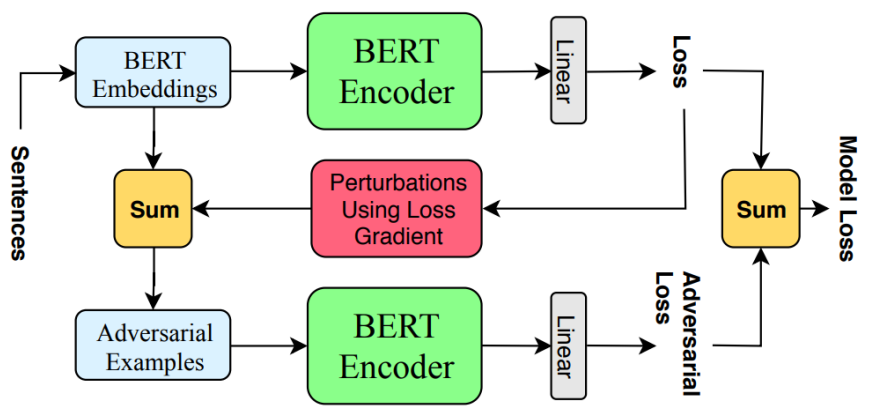
\includegraphics[keepaspectratio, width=0.45\textwidth]{pics/1.png}}
\caption{A representation of the model used by A. Karimi et al.}
\label{fig}
\end{figure}

\begin{figure*}
\centerline{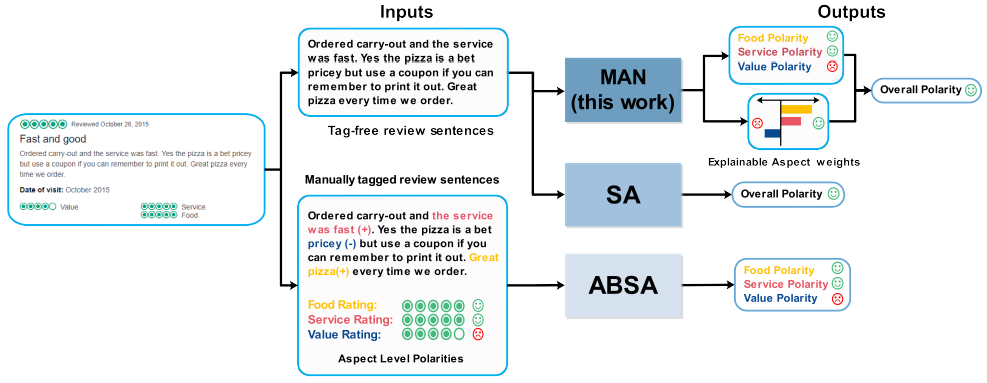
\includegraphics[keepaspectratio, width=\textwidth]{pics/2.png}}
  \caption{A summary of the aims of Y. Qiang at al in this paper.}
\end{figure*}

For the AE subtask, the goal was to assign each word a label so as to specify whether it is the beginning of an aspect, inside an aspect or not in any aspect. For the ASC subtask, the output from the previous subtask is used as input (in the evaluation stage, while the actual true values are utilized in training) with the modification that each text is repeated as many times as there are aspects in it so that the setiment for each aspect can be classified separately.

The hyperparameter to be optimized is the variable that controls how big the perturbations being added to the input sample are. The challenge with optimizing that was that the adversarial sample to be produced needed to be similar enough to the input to be classified as the same but also different enough from the input so as to challenge the model. The issue that the authors faced is that they were using 2 distinct datasets but the best value that they found was different for both meaning that the dataset itself influences the best value for this parameter.

Furthermore, as the authors were buiding upon another research on the same topic but using a post-trained BERT (BERT-PT), they had to keep many things in their paper and methodology consistent with that approach. This means that their paper is easy to compare with other approaches but it seems there was still room for further experimentation for their approach as it was constrained so as to be comparable.


\begin{table}[htbp]
\caption{Results of the model produced by Y. Qiang et al.}
\begin{center}
\begin{tabular}{|c|c|c|c|}
\hline
\multicolumn{2}{|c|}{\textbf{Restaurant}} & \multicolumn{2}{|c|}{\textbf{Laptop}} \\
\hline
\textbf{AE} & \textbf{ASC} & \textbf{AE} & \textbf{ASC} \\
\hline
80.9 & 85.4 & 85.6 & 78.1 \\
\hline
\end{tabular}
\end{center}
\end{table}


The results were indeed an improvement upon BERT-PT and it can be said that they had produced the best results at the time for the given datasets.\\

\textit{\textbf{Toward Tag-free Aspect Based Sentiment Analysis:
A Multiple Attention Network Approach, Y. Qiang et al, 2020.}}

This paper identifies the issue that datasets for ABSA need to have the aspects tagged manually, which leads to their being less relevant data available even though there is a very large number of review and opinion texts available online today. This is refered to as the cold-start problem. They propose a new Multiple-Attention Network (MAN) approach which crawls the review data from review websites to extract the tag-free review text, aspect-level ratings, and overall ratings. Their aim is to provide an end-to-end automatic solution to perform ABSA as well as to uncover the weighted contribution of each word towards the aspect-level and overall polarities. A summary of their aim is provided by Figure 2.

The contributions of this work are combatting the cold-start for ABSA models by creating a means to produce datasets from review websites, providing 2 new datasets made from TripAdvisor, and including a means of inferring the overall sentiment from the aspect polarities by identifying the contribution of each aspect towards the overall score. The paper comments that a lot of ABSA approaches are built on SemEval Task5, and the authors want a greater use of the massive online review data being generated from e-commerce websites by alleviating the laborious process of manually tagging the available reviews.

\begin{figure}[htbp]
\centerline{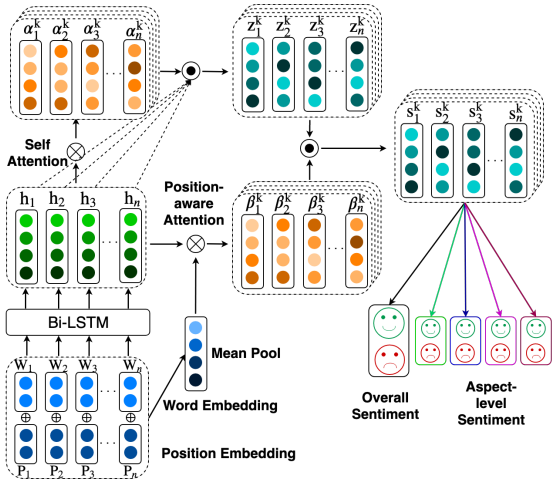
\includegraphics[keepaspectratio, width=0.5\textwidth]{pics/3.png}}
\caption{A representation of the model used by Y. Qiang et al.}
\label{fig}
\end{figure}

The authors provide 2 datasets, one for hotel ratings and the other for restaurant ratings, which they have produced by scraping reviews from TripAdvisor. As shown in Figure 3, the MAN model consists of a number of modules. In the model, the sentences are embedded into word vectors those vectors are combined with their positional information. The input is then parsed into a Bi-LSTM to produce hidden states for each word. Self-attention is then performed to produce allignment vectors for each word for each aspect which are combined with the original hidden states to produce the context vectors for each word.

Position-aware self attention is also performed as words which are closer to an aspect will have more relevance to it usually. These arrays of vectors are also produced for each aspect. Thus we get another set of position-aware alignment vectors. These are combined with the context vectors to give the final representaions of the aspects which can then be classified. The classification is performed overall as well as on each aspect on a positive or negative class bases.

Several standard pre-processing techniques, such as lemmatization, stemming, stop word removal and tokenization are used so as to reduce the number of words and to make the process more efficient. Also, the attention scores are used to derive the more important aspects from a text, which is then used to give more weightage to it when calculating the overall polarity.

\begin{table}[htbp]
\caption{Results of the model produced by Y. Qiang et al.}
\begin{center}
\begin{tabular}{|c|c|c|c|}
\hline
\multicolumn{2}{|c|}{\textbf{Restaurant}} & \multicolumn{2}{|c|}{\textbf{Hotel}} \\
\hline
\textbf{ACC} & \textbf{Macro-F1} & \textbf{ACC} & \textbf{Macro-F1} \\
\hline
89.64±0.18 & 77.60±0.26 & 83.06±0.14 & 79.81±0.22 \\
\hline
\end{tabular}
\end{center}
\end{table}

From the results above we can see that the model produced sufficiently high accuracy given the fact that the input data was unstructured and scraped off from a review website. And this paper has been successful in addressing the cold-start problem which it aimed to solve. Furthermore, it has introduced a method to build end-to-end ABSA solutions for unstructured data, which without doubt will be expanded upon in the future.\\

\textit{\textbf{Aspect-based Sentiment Analysis with
Type-aware Graph Convolutional Networks and Layer Ensemble, Y. Tian et al, 2021.}}

This paper talks about a better way of using dependancy parsing in ABSA. Previous implementations have used dependancy graphs for text to assist in performing ABSA for that text, but only the dependancies have been paid attention to, not the exact type of dependancy among the words. Clearly some dependancies such as the one between a noun and a verb in a simple sentence are more important in ascertaining the polarity of an aspect within a text as compared with other dependancies that exist within that sentence. If all dependancies are treated equally, this will clearly be a disadvantageous for the model in performing ABSA.

Additionally, this paper claims that although previous Graph Convolutional Networks (GCNs) have learned relations using multiple layers, they only use the result from the most recent layer for ABSA which leads to some being lost because different contextual information is present in different layers in an ensemble.

This paper investigates a Type-Aware Graph Convolutional Network (T-GCN) with multiple layers incorporating both word relational information and dependancy type information so as to improve on the current approaches for ABSA. The overall architecture for their approach is given by Figure 4.

\begin{figure}[htbp]
\centerline{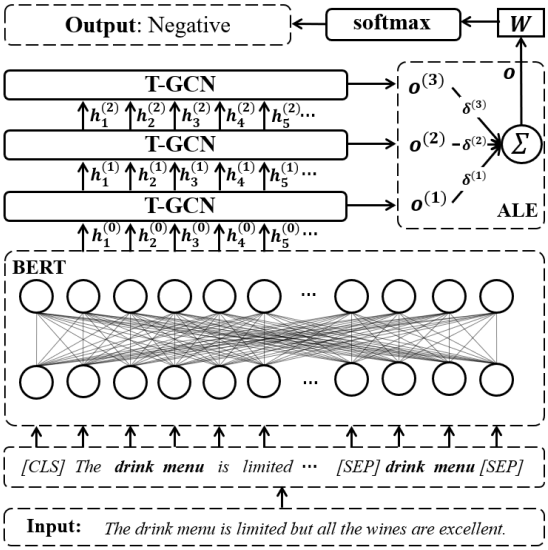
\includegraphics[keepaspectratio, width=0.5\textwidth]{pics/4.png}}
\caption{The overall representation of the model used by Y. Tian et al.}
\label{fig}
\end{figure}

First, given an input sentence, off-the-shelf toolkits are used to get the dependancy information. From this information an adjacency matrix is made to show the relation information of the dependancy graph, and relation matrix is made to show the type information, as shown in Figure 5. The sentence along with the provided aspect information is tokenized and then the resultant words are vectorized and put through a BERT to get the relevant attention information.

\begin{figure}[htbp]
\centerline{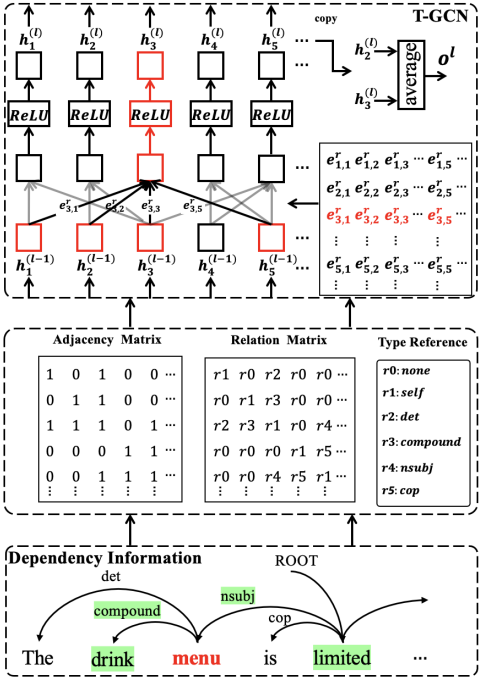
\includegraphics[keepaspectratio, width=0.5\textwidth]{pics/5.png}}
\caption{An illustration of how the type-aware graph is built and how each layer in the T-GCN processes the hidden states.}
\label{fig}
\end{figure}

The graph and the hidden states are then input to the T-GCN where a transition matrix is used to map the relations to their embeddings. For each edge, each layer in the T-GCN first combines the hidden vector with its relational embedding, then the results for the two words connected by the edge are combined and the weight of this edge is calculated. The trainable weight matrix for that layer is then used to produce the intermediate hidden state. Finally, the weight of the edge is applied to the hidden state, and a ReLU activation is performed to produce the hidden state output. This output is then the input for the next layer.

For each word, every layer incorporates information from its connected words into it, this means that multiple layers could learn longer and complex relations. This paper proposes to thus study this contextual information from all the layers using an Attentive Layer Ensemble (ALE). The hidden vectors from each layer are summed and averaged with respect to the number of aspect terms that were initially provided to provide an output from each layer. A weighted average of these output vectors is then taken which is the final output vector for ABSA.

A fully connected layer is then used to map this output vector to the number of classes and then softmax activation is applied to predict the output sentiment for the aspect.

The model showed better accuracy as compared to other famous studies operating on the same datasets. The authors also portrayed which exact studies were utilizing dependancy information in their comparision. It is interesting to note that most of the studies with higher performance were using dependancy information in some form. This points to the reasoning that exploring the direction of incorporating dependancy type information to improve ABSA models might be the direction to go in in the future. The authors have also provided evidence that usng T-GCN and ALE both have lead to some improvements in the accuracy of the models.

\subsection{2020-2023}

\section{Prepare Your Paper Before Styling}
Before you begin to format your paper, first write and save the content as a 
separate text file. Complete all content and organizational editing before 
formatting. Please note sections \ref{AA}--\ref{SCM} below for more information on 
proofreading, spelling and grammar.

Keep your text and graphic files separate until after the text has been 
formatted and styled. Do not number text heads---{\LaTeX} will do that 
for you.

\subsection{Abbreviations and Acronyms}\label{AA}
Define abbreviations and acronyms the first time they are used in the text, 
even after they have been defined in the abstract. Abbreviations such as 
IEEE, SI, MKS, CGS, ac, dc, and rms do not have to be defined. Do not use 
abbreviations in the title or heads unless they are unavoidable.

\subsection{Units}
\begin{itemize}
\item Use either SI (MKS) or CGS as primary units. (SI units are encouraged.) English units may be used as secondary units (in parentheses). An exception would be the use of English units as identifiers in trade, such as ``3.5-inch disk drive''.
\item Avoid combining SI and CGS units, such as current in amperes and magnetic field in oersteds. This often leads to confusion because equations do not balance dimensionally. If you must use mixed units, clearly state the units for each quantity that you use in an equation.
\item Do not mix complete spellings and abbreviations of units: ``Wb/m\textsuperscript{2}'' or ``webers per square meter'', not ``webers/m\textsuperscript{2}''. Spell out units when they appear in text: ``. . . a few henries'', not ``. . . a few H''.
\item Use a zero before decimal points: ``0.25'', not ``.25''. Use ``cm\textsuperscript{3}'', not ``cc''.)
\end{itemize}

\subsection{Equations}
Number equations consecutively. To make your 
equations more compact, you may use the solidus (~/~), the exp function, or 
appropriate exponents. Italicize Roman symbols for quantities and variables, 
but not Greek symbols. Use a long dash rather than a hyphen for a minus 
sign. Punctuate equations with commas or periods when they are part of a 
sentence, as in:
\begin{equation}
a+b=\gamma\label{eq}
\end{equation}

Be sure that the 
symbols in your equation have been defined before or immediately following 
the equation. Use ``\eqref{eq}'', not ``Eq.~\eqref{eq}'' or ``equation \eqref{eq}'', except at 
the beginning of a sentence: ``Equation \eqref{eq} is . . .''

\subsection{\LaTeX-Specific Advice}

Please use ``soft'' (e.g., \verb|\eqref{Eq}|) cross references instead
of ``hard'' references (e.g., \verb|(1)|). That will make it possible
to combine sections, add equations, or change the order of figures or
citations without having to go through the file line by line.

Please don't use the \verb|{eqnarray}| equation environment. Use
\verb|{align}| or \verb|{IEEEeqnarray}| instead. The \verb|{eqnarray}|
environment leaves unsightly spaces around relation symbols.

Please note that the \verb|{subequations}| environment in {\LaTeX}
will increment the main equation counter even when there are no
equation numbers displayed. If you forget that, you might write an
article in which the equation numbers skip from (17) to (20), causing
the copy editors to wonder if you've discovered a new method of
counting.

{\BibTeX} does not work by magic. It doesn't get the bibliographic
data from thin air but from .bib files. If you use {\BibTeX} to produce a
bibliography you must send the .bib files. 

{\LaTeX} can't read your mind. If you assign the same label to a
subsubsection and a table, you might find that Table I has been cross
referenced as Table IV-B3. 

{\LaTeX} does not have precognitive abilities. If you put a
\verb|\label| command before the command that updates the counter it's
supposed to be using, the label will pick up the last counter to be
cross referenced instead. In particular, a \verb|\label| command
should not go before the caption of a figure or a table.

Do not use \verb|\nonumber| inside the \verb|{array}| environment. It
will not stop equation numbers inside \verb|{array}| (there won't be
any anyway) and it might stop a wanted equation number in the
surrounding equation.

\subsection{Some Common Mistakes}\label{SCM}
\begin{itemize}
\item The word ``data'' is plural, not singular.
\item The subscript for the permeability of vacuum $\mu_{0}$, and other common scientific constants, is zero with subscript formatting, not a lowercase letter ``o''.
\item In American English, commas, semicolons, periods, question and exclamation marks are located within quotation marks only when a complete thought or name is cited, such as a title or full quotation. When quotation marks are used, instead of a bold or italic typeface, to highlight a word or phrase, punctuation should appear outside of the quotation marks. A parenthetical phrase or statement at the end of a sentence is punctuated outside of the closing parenthesis (like this). (A parenthetical sentence is punctuated within the parentheses.)
\item A graph within a graph is an ``inset'', not an ``insert''. The word alternatively is preferred to the word ``alternately'' (unless you really mean something that alternates).
\item Do not use the word ``essentially'' to mean ``approximately'' or ``effectively''.
\item In your paper title, if the words ``that uses'' can accurately replace the word ``using'', capitalize the ``u''; if not, keep using lower-cased.
\item Be aware of the different meanings of the homophones ``affect'' and ``effect'', ``complement'' and ``compliment'', ``discreet'' and ``discrete'', ``principal'' and ``principle''.
\item Do not confuse ``imply'' and ``infer''.
\item The prefix ``non'' is not a word; it should be joined to the word it modifies, usually without a hyphen.
\item There is no period after the ``et'' in the Latin abbreviation ``et al.''.
\item The abbreviation ``i.e.'' means ``that is'', and the abbreviation ``e.g.'' means ``for example''.
\end{itemize}
An excellent style manual for science writers is \cite{b7}.

\subsection{Authors and Affiliations}
\textbf{The class file is designed for, but not limited to, six authors.} A 
minimum of one author is required for all conference articles. Author names 
should be listed starting from left to right and then moving down to the 
next line. This is the author sequence that will be used in future citations 
and by indexing services. Names should not be listed in columns nor group by 
affiliation. Please keep your affiliations as succinct as possible (for 
example, do not differentiate among departments of the same organization).

\subsection{Identify the Headings}
Headings, or heads, are organizational devices that guide the reader through 
your paper. There are two types: component heads and text heads.

Component heads identify the different components of your paper and are not 
topically subordinate to each other. Examples include Acknowledgments and 
References and, for these, the correct style to use is ``Heading 5''. Use 
``figure caption'' for your Figure captions, and ``table head'' for your 
table title. Run-in heads, such as ``Abstract'', will require you to apply a 
style (in this case, italic) in addition to the style provided by the drop 
down menu to differentiate the head from the text.

Text heads organize the topics on a relational, hierarchical basis. For 
example, the paper title is the primary text head because all subsequent 
material relates and elaborates on this one topic. If there are two or more 
sub-topics, the next level head (uppercase Roman numerals) should be used 
and, conversely, if there are not at least two sub-topics, then no subheads 
should be introduced.

\subsection{Figures and Tables}
\paragraph{Positioning Figures and Tables} Place figures and tables at the top and 
bottom of columns. Avoid placing them in the middle of columns. Large 
figures and tables may span across both columns. Figure captions should be 
below the figures; table heads should appear above the tables. Insert 
figures and tables after they are cited in the text. Use the abbreviation 
``Fig.~\ref{fig}'', even at the beginning of a sentence.

\begin{table}[htbp]
\caption{Table Type Styles}
\begin{center}
\begin{tabular}{|c|c|c|c|}
\hline
\textbf{Table}&\multicolumn{3}{|c|}{\textbf{Table Column Head}} \\
\cline{2-4} 
\textbf{Head} & \textbf{\textit{Table column subhead}}& \textbf{\textit{Subhead}}& \textbf{\textit{Subhead}} \\
\hline
copy& More table copy$^{\mathrm{a}}$& &  \\
\hline
\multicolumn{4}{l}{$^{\mathrm{a}}$Sample of a Table footnote.}
\end{tabular}
\label{tab1}
\end{center}
\end{table}

\begin{figure}[htbp]
\centerline{Picture here}
\caption{Example of a figure caption.}
\label{fig}
\end{figure}

Figure Labels: Use 8 point Times New Roman for Figure labels. Use words 
rather than symbols or abbreviations when writing Figure axis labels to 
avoid confusing the reader. As an example, write the quantity 
``Magnetization'', or ``Magnetization, M'', not just ``M''. If including 
units in the label, present them within parentheses. Do not label axes only 
with units. In the example, write ``Magnetization (A/m)'' or ``Magnetization 
\{A[m(1)]\}'', not just ``A/m''. Do not label axes with a ratio of 
quantities and units. For example, write ``Temperature (K)'', not 
``Temperature/K''.

\section*{Acknowledgment}

The preferred spelling of the word ``acknowledgment'' in America is without 
an ``e'' after the ``g''. Avoid the stilted expression ``one of us (R. B. 
G.) thanks $\ldots$''. Instead, try ``R. B. G. thanks$\ldots$''. Put sponsor 
acknowledgments in the unnumbered footnote on the first page.

\section*{References}

Please number citations consecutively within brackets \cite{b1}. The 
sentence punctuation follows the bracket \cite{b2}. Refer simply to the reference 
number, as in \cite{b3}---do not use ``Ref. \cite{b3}'' or ``reference \cite{b3}'' except at 
the beginning of a sentence: ``Reference \cite{b3} was the first $\ldots$''

Number footnotes separately in superscripts. Place the actual footnote at 
the bottom of the column in which it was cited. Do not put footnotes in the 
abstract or reference list. Use letters for table footnotes.

Unless there are six authors or more give all authors' names; do not use 
``et al.''. Papers that have not been published, even if they have been 
submitted for publication, should be cited as ``unpublished'' \cite{b4}. Papers 
that have been accepted for publication should be cited as ``in press'' \cite{b5}. 
Capitalize only the first word in a paper title, except for proper nouns and 
element symbols.

For papers published in translation journals, please give the English 
citation first, followed by the original foreign-language citation \cite{b6}.

\begin{thebibliography}{00}
\bibitem{b1} G. Eason, B. Noble, and I. N. Sneddon, ``On certain integrals of Lipschitz-Hankel type involving products of Bessel functions,'' Phil. Trans. Roy. Soc. London, vol. A247, pp. 529--551, April 1955.
\bibitem{b2} J. Clerk Maxwell, A Treatise on Electricity and Magnetism, 3rd ed., vol. 2. Oxford: Clarendon, 1892, pp.68--73.
\bibitem{b3} I. S. Jacobs and C. P. Bean, ``Fine particles, thin films and exchange anisotropy,'' in Magnetism, vol. III, G. T. Rado and H. Suhl, Eds. New York: Academic, 1963, pp. 271--350.
\bibitem{b4} K. Elissa, ``Title of paper if known,'' unpublished.
\bibitem{b5} R. Nicole, ``Title of paper with only first word capitalized,'' J. Name Stand. Abbrev., in press.
\bibitem{b6} Y. Yorozu, M. Hirano, K. Oka, and Y. Tagawa, ``Electron spectroscopy studies on magneto-optical media and plastic substrate interface,'' IEEE Transl. J. Magn. Japan, vol. 2, pp. 740--741, August 1987 [Digests 9th Annual Conf. Magnetics Japan, p. 301, 1982].
\bibitem{b7} M. Young, The Technical Writer's Handbook. Mill Valley, CA: University Science, 1989.
\end{thebibliography}
\vspace{12pt}
\color{red}
IEEE conference templates contain guidance text for composing and formatting conference papers. Please ensure that all template text is removed from your conference paper prior to submission to the conference. Failure to remove the template text from your paper may result in your paper not being published.

\end{document}